\setcounter{equation}{0}

\nomenclature{}{}

\chapter{Overview}

The Kolmogorov-Arnold Network (KAN) model is a novel deep learning architecture inspired by the Kolmogorov-Arnold representation theorem. This theorem suggests that any continuous, multivariate function can be represented as a composition of univariate functions. KAN leverages this idea by replacing the fixed activation functions on nodes ("neurons") seen in traditional Multi-Layer Perceptrons (MLPs) with learnable activation functions on edges ("weights"). 
\begin{figure}[t]
    \centering
    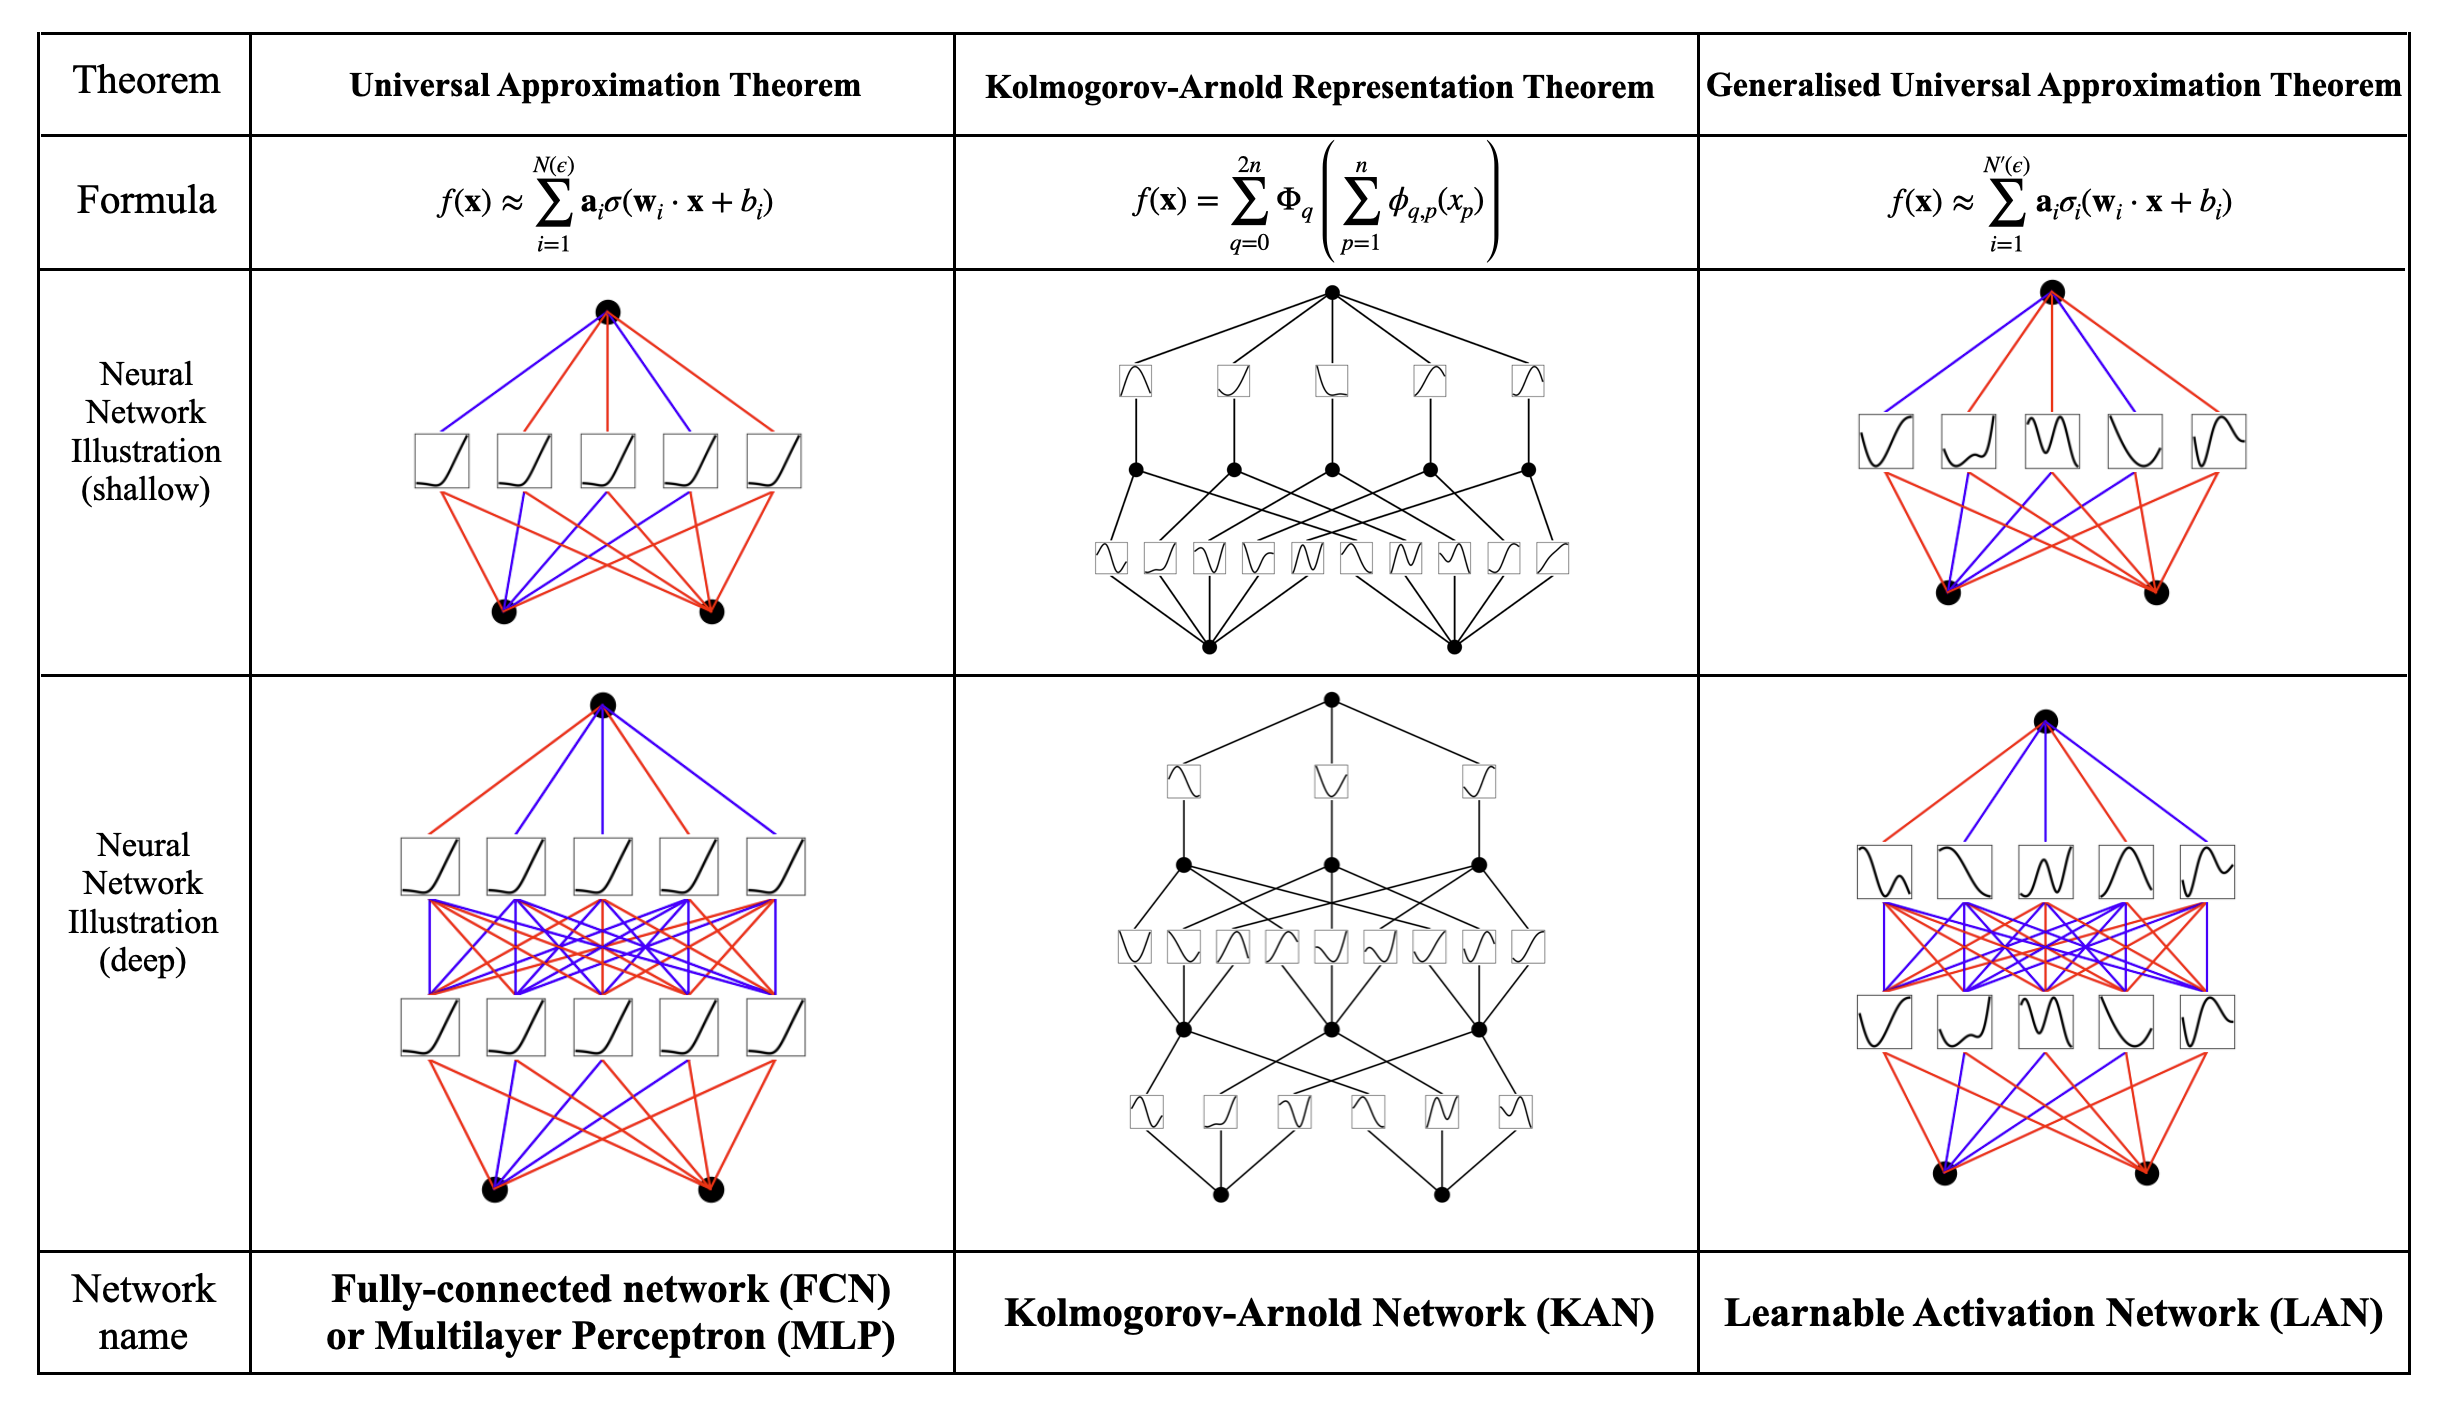
\includegraphics[width=1\linewidth]{Images/theory_model.png}
    \caption{Multi-Layer Perceptrons (MLPs) vs. Kolmogorov-Arnold Networks (KANs)}
\end{figure}

This fundamental difference eliminates linear weight matrices, with each weight parameter becoming a learnable 1D function, typically parameterized as a spline. KAN nodes perform simple summation without non-linearities.
\\
The primary objectives of the KAN model are:

\begin{itemize}
    \item Accuracy: KANs aim to achieve higher accuracy in function fitting tasks compared to MLPs, particularly for functions with compositional structures. Their ability to optimize learned features to great accuracy due to the use of splines is a key factor. Empirical evidence suggests KANs may exhibit faster neural scaling laws and better generalization capabilities than MLPs.
    \item Interpretability: KANs are designed for enhanced interpretability. The visualization of activation functions as 1D curves allows for intuitive understanding of feature relationships and their contribution to the output. Techniques like sparsification and pruning further enhance interpretability by simplifying the network structure and enabling the extraction of symbolic formulas from trained KANs.
\end{itemize}

\begin{figure}[t]
    \centering
    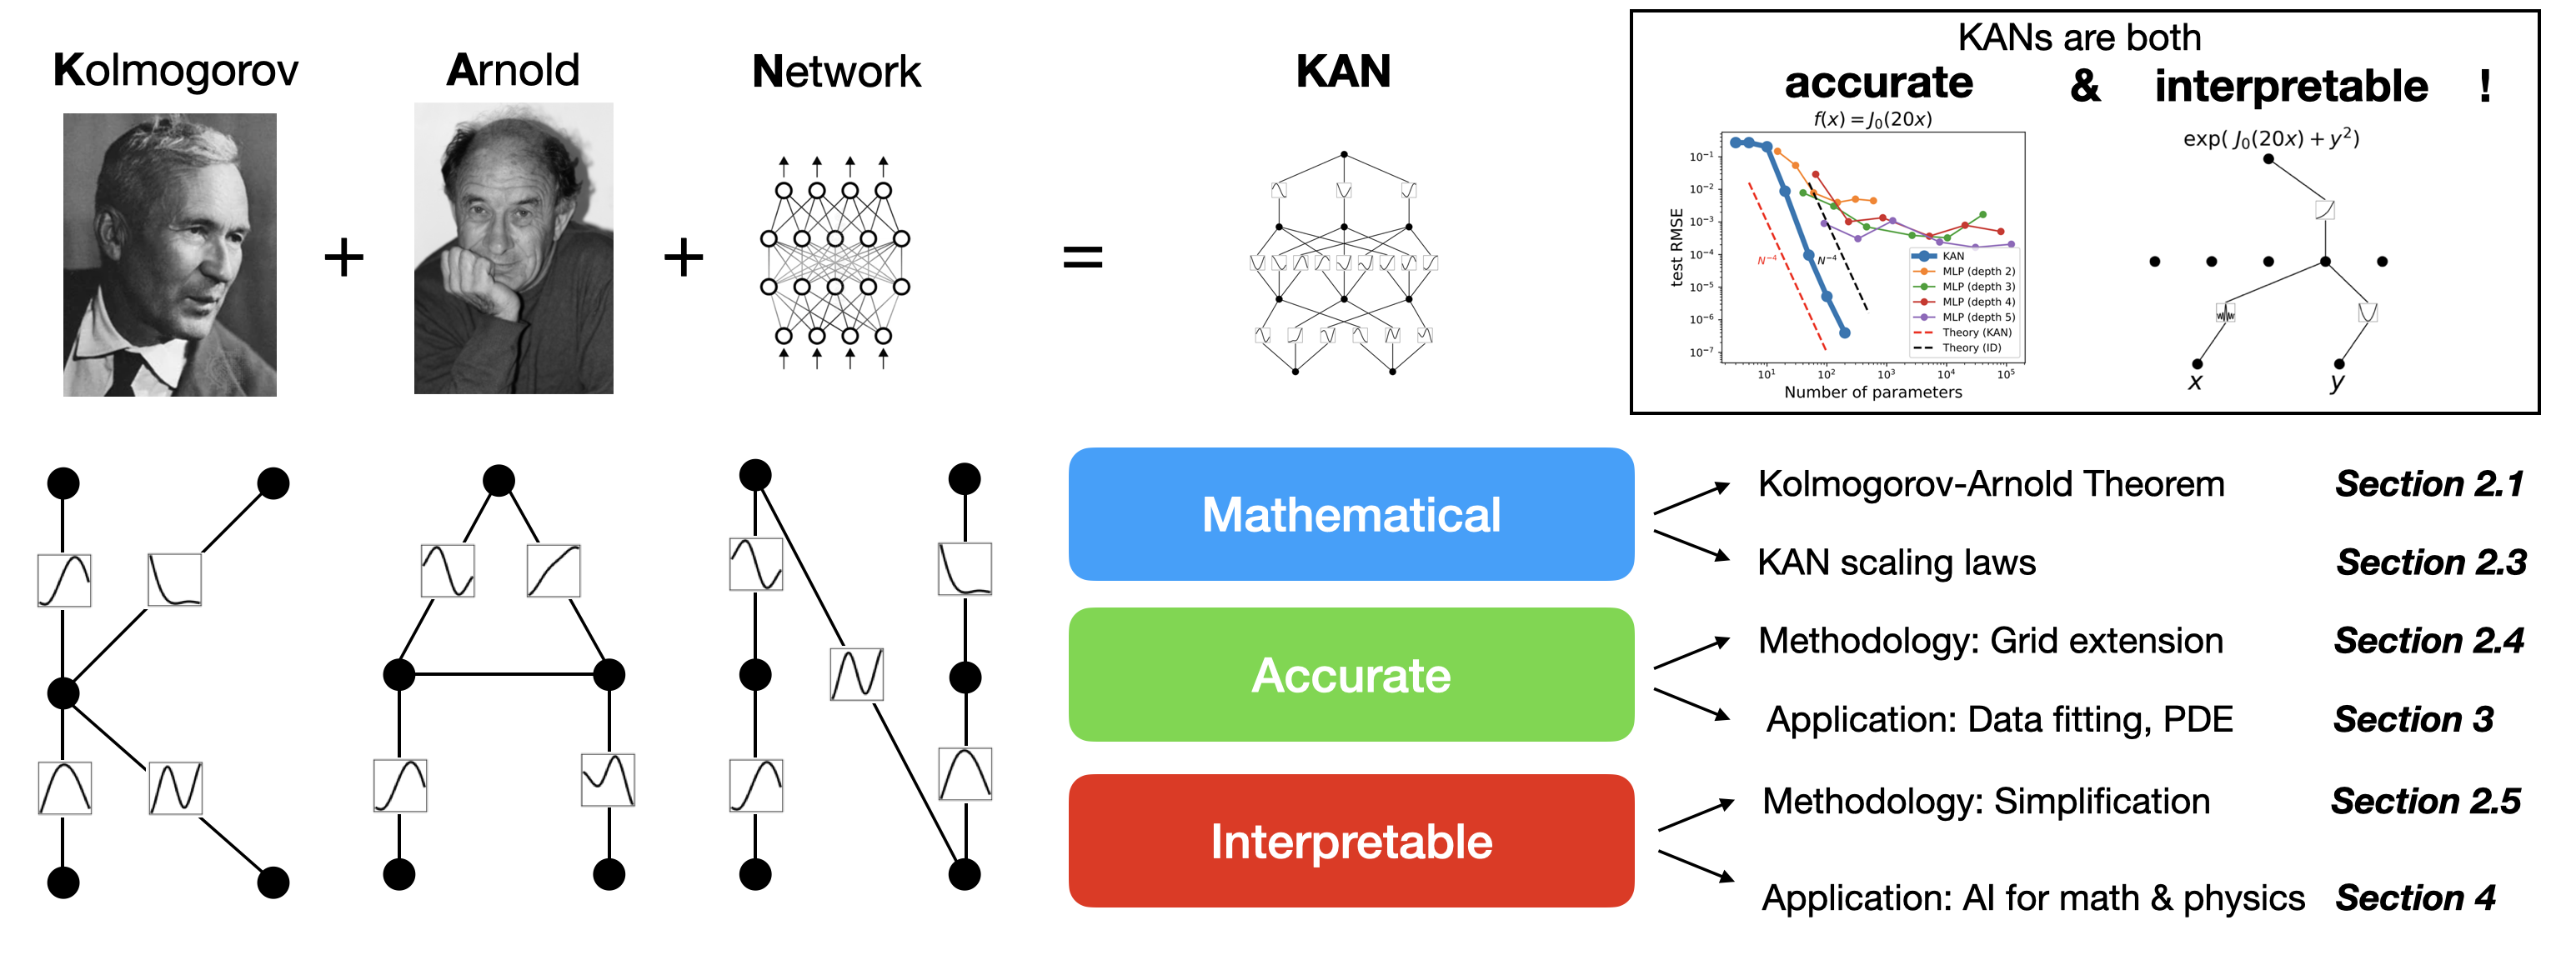
\includegraphics[width=1\linewidth]{Images/flowchart.png}
    \caption{Kolmogorov-Arnold networks are in honor of two great late mathematicians, Andrey Kolmogorov and Vladimir Arnold. KANs are mathematically sound, accurate and interpretable.}
\end{figure}

It is important to note that, while promising, the research surrounding KANs is still in its early stages. Some studies have shown that KANs may not outperform MLPs in all tasks and domains. The computational cost of training KANs can also be significantly higher than that of MLPs. Further research is needed to address these limitations and fully unlock the potential of KANs across diverse applications.